\section{Experiments}
\begin{frame}
    \frametitle{Experiments}
    \framesubtitle{Details of the hardware}

    \begin{center}
        \begin{tabular}{lr}
            \hline
            {CPU} & Intel(R) Xeon(R) CPU E5-4650 0 @ 2.70GHz \\
            {GPU} & Tesla M2050 @ 575 Mhz (448 cores). \\
            {RAM} & 24 GB \\
            {OS}  & Scientific Linux release 6.4 \\
            \hline
        \end{tabular}
    \end{center}
\end{frame}

\begin{frame}
    \frametitle{Experiments}
    \framesubtitle{Integrator scaling}

\begin{figure}[H]
    \centering
    \label{fig:time}
    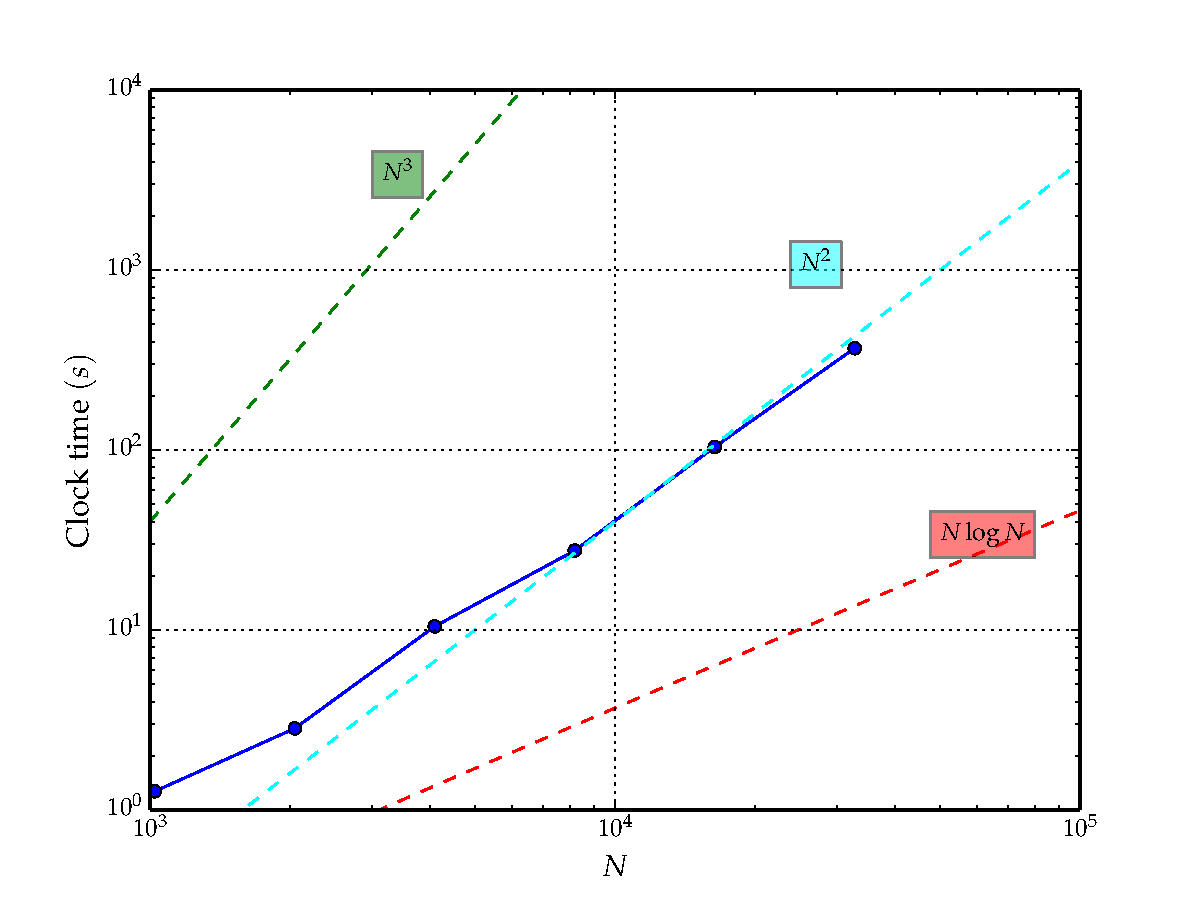
\includegraphics[width=0.65\textwidth]{img/test_time-1t-N.pdf}
    \caption{Clock time of integration from $t=1$ to $t=2$ NBU using $\eta = 0.01$ and
             $\epsilon = 10^{-4}$ using different amount of particles.}
\end{figure}

\end{frame}

\begin{frame}
    \frametitle{Experiments}
    \framesubtitle{Clock time comparison}

\begin{table}[H]
    \centering
    \footnotesize
    \begin{tabular}{rrrrrrr}
        \hline
        {\bf N} & \multicolumn{1}{c}{\bf CPU}
                & \multicolumn{1}{c}{\bf OpenMP}
                & \multicolumn{1}{c}{\bf CPU + GPU}
                & \multicolumn{1}{c}{\bf MPI-1}
                & \multicolumn{1}{c}{\bf MPI-2}
                & \multicolumn{1}{c}{\bf GPU}   \\
         %{\bf  1k} &    12.98 [s] &     8.19 [s]  &    3.57 [s]      &    6.17 [s] &    2.68 [s] &    1.21 [s]          \\
         %{\bf  2k} &    61.32 [s] &    34.94 [s]  &   13.42 [s]      &   14.51 [s] &    7.34 [s] &    3.22 [s]          \\
         %{\bf  4k} &   282.98 [s] &   162.64 [s]  &   54.28 [s]      &   51.14 [s] &   27.12 [s] &    9.45 [s]          \\
         %{\bf  8k} &  1227.40 [s] &   682.56 [s]  &  208.91 [s]      &  105.65 [s] &   64.61 [s] &   23.31 [s]          \\
         %{\bf 16k} &  5542.35 [s] &  3227.91 [s]  &  904.82 [s]      &  364.90 [s] &  317.51 [s] &   82.63 [s]          \\
         %{\bf 32k} & 26383.71 [s] & 15076.40 [s]  & 3722.92 [s]      & 1247.33 [s] & 1145.82 [s] &  275.53 [s]          \\ \hline
         {\bf  1k} &    12 &     8  &    3      &    6  &    2 &    1          \\
         {\bf  2k} &    61 &    34  &   13      &   14  &    7 &    3          \\
         {\bf  4k} &   282 &   162  &   54      &   51  &   27 &    9          \\
         {\bf  8k} &  1227 &   682  &  208      &  105  &   64 &   23          \\
         {\bf 16k} &  5542 &  3227  &  904      &  364  &  317 &   82          \\
         {\bf 32k} & 26383 & 15076  & 3722      & 1247  & 1145 &  275          \\ \hline
    \end{tabular}
    \caption{Clock time foreach integrator version (in sec).}
    \label{tab:acc}
\end{table}

\end{frame}

\begin{frame}
    \frametitle{Experiments}
    \framesubtitle{Clock time comparison}

\begin{figure}[H]
    \centering
    \label{fig:acc}
    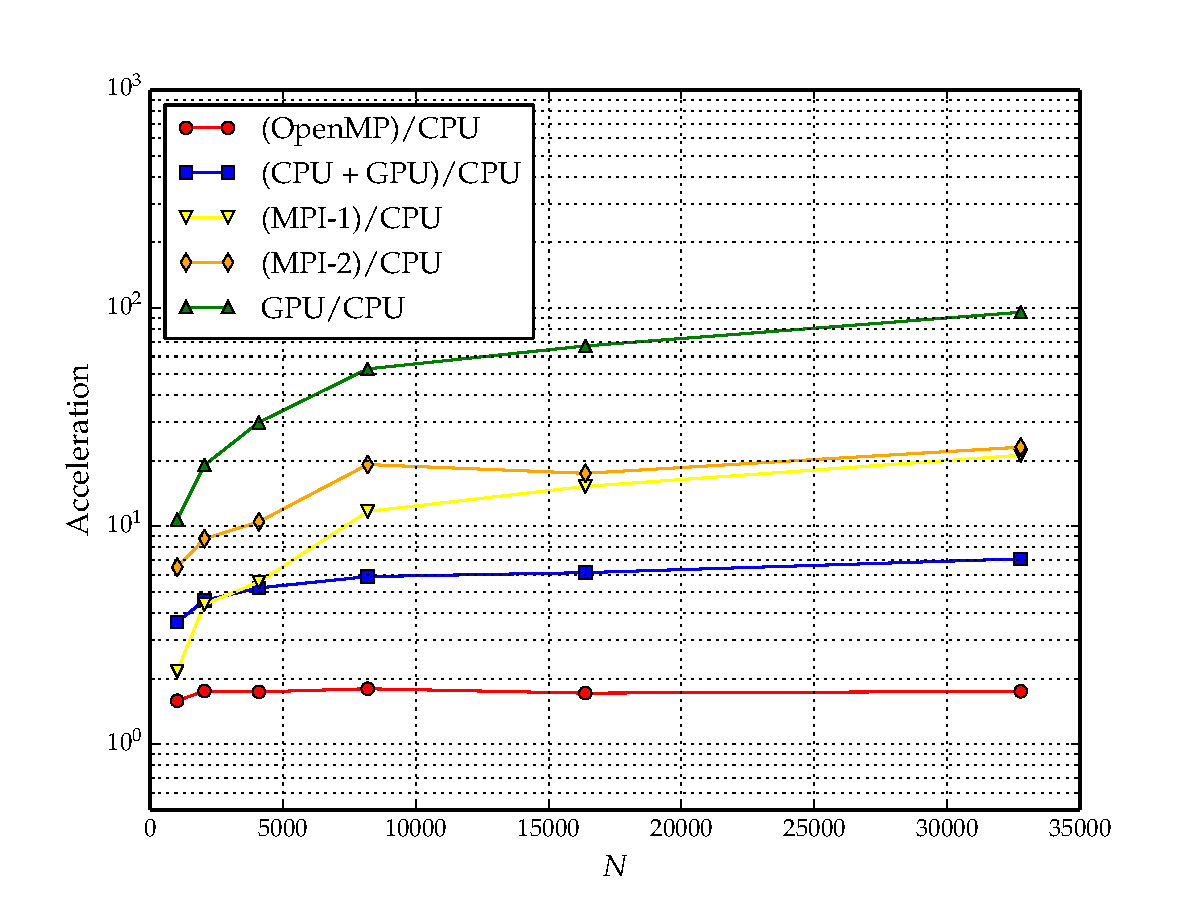
\includegraphics[width=0.8\textwidth]{img/test_gpu-acceleration.pdf}
    \caption{Acceleration between the implementations described in Table~\ref{tab:acc}}
\end{figure}

\end{frame}
\begin{frame}
    \frametitle{Experiments}
    \framesubtitle{Integrator Performance}
\begin{figure}[H]
    \centering
    \label{fig:gflops}
    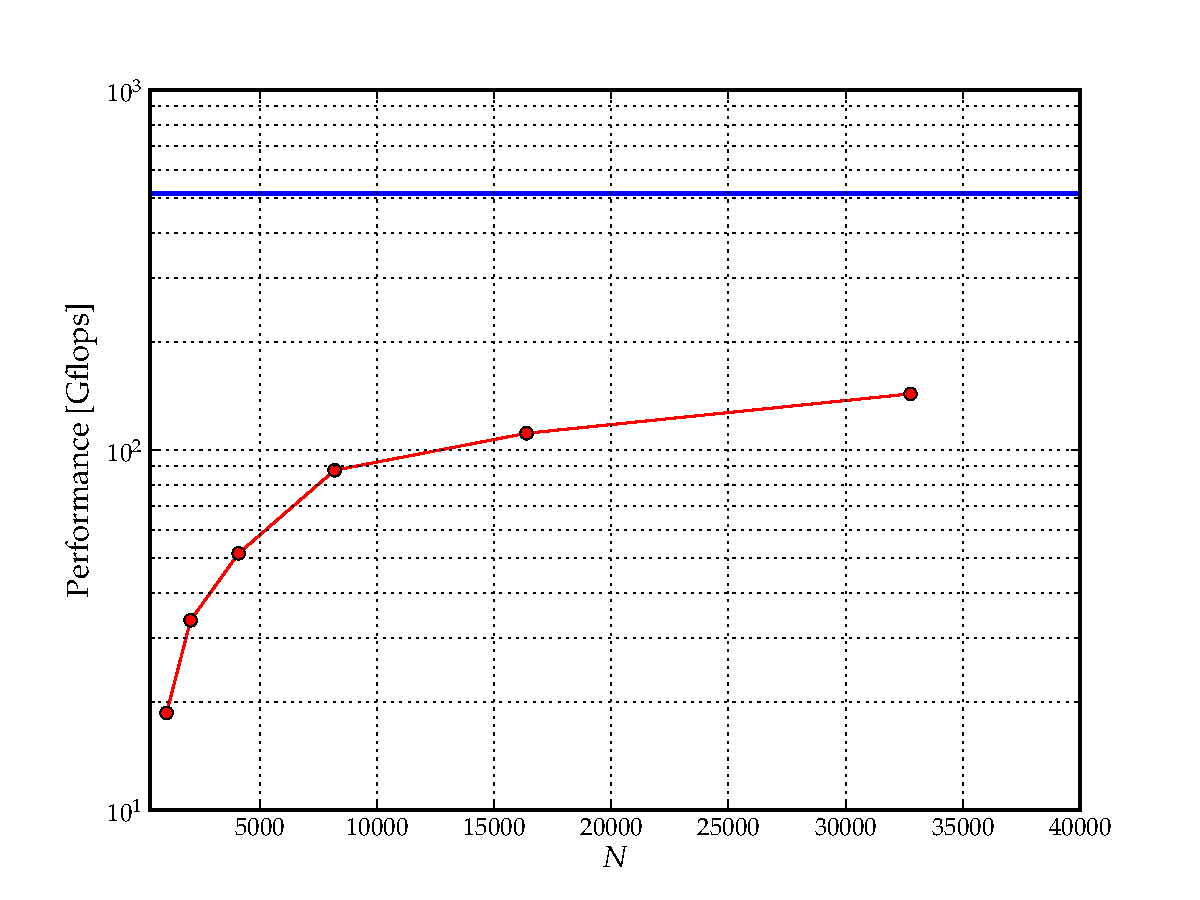
\includegraphics[width=0.65\textwidth]{img/test_gflops.pdf}
    \caption{GPU gravitational interactions performance in GFLOPS for different amount of particles.}
\end{figure}

\end{frame}
